\section{StarDICE response}
\label{sec:rsd}

In this section, we will show the methodology to obtain the \SD telescope response $\Rtel(\lambda)$ by analyzing \SD camera data.

\subsection{Data set description and strategy}
\label{sec:sd_datadesc}

As described in section \ref{sec:cbp_datadesc}, the laser emits pulses at a rate of \SI{1}{\kilo\hertz} in bursts that are separated with dark times. We set the \spinhole pinhole to measure the \SD throughput and its filter transmissions. Yet, as discussed in Section~\ref{sec:strategy} the calibration of the CBP throughput is obtained with the \bpinhole pinhole, so we use an open transmission measurement of the \SD telescope with both pinholes to intercalibrate the CBP and \SD telescope responses. Figure~\ref{fig:ccd_examples} shows examples of images obtained when the CBP shoots in the \SD CCD camera with two different pinholes. \\

In the following sections, we describe the modelization of the \spinhole pinhole dataset via PSF photometry. Then, we discuss the choice of the baseline photometry used to measure the \SD response, and the method to intercalibrate it with the CBP response. Finally we will show the result obtained.

\begin{figure}[h]
    \centering
    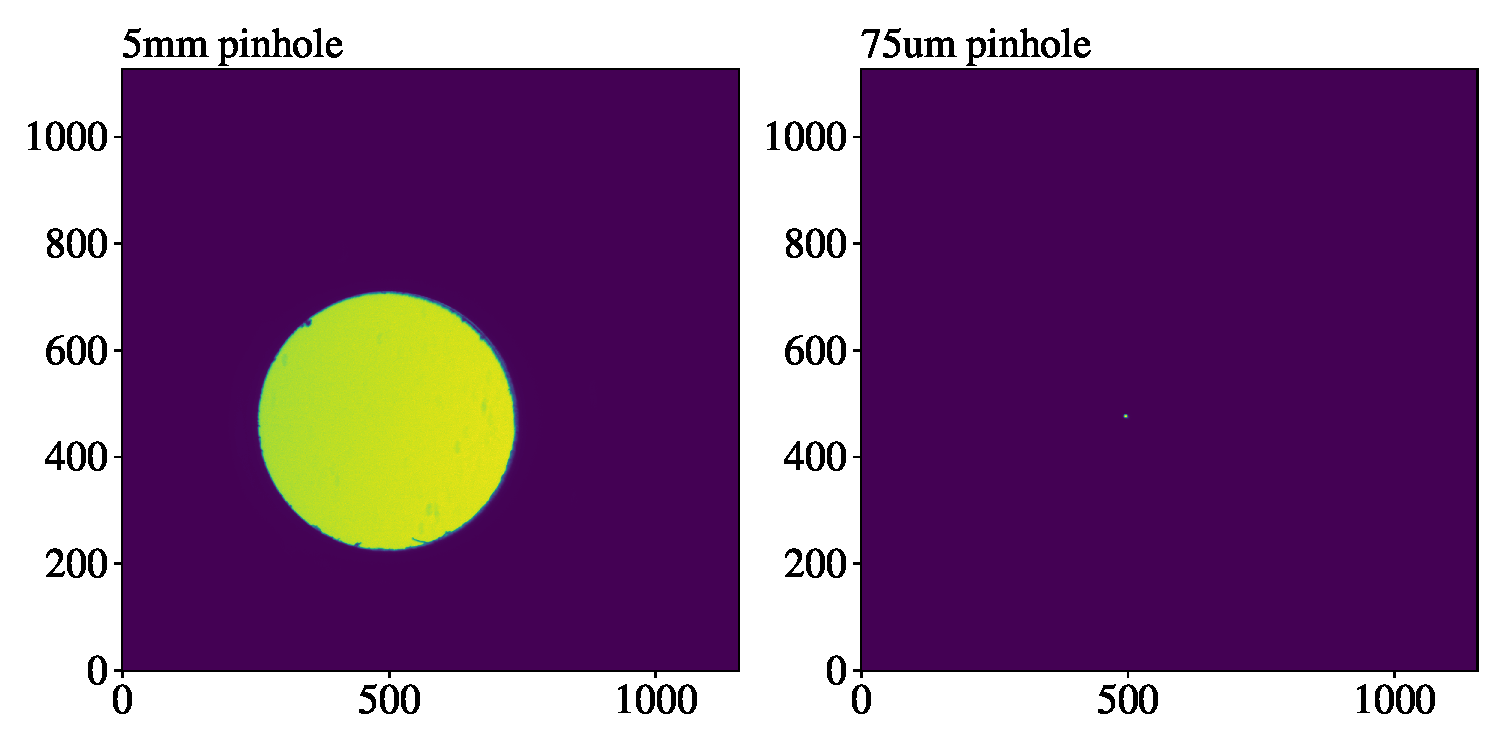
\includegraphics[width=\columnwidth]{fig/ccd_examples.pdf}
    \caption{Examples of images obtained when the CBP shoots in the \SD telescope at $\lambda_L=\SI{450}{\nm}$ with the \bpinhole pinhole on the right and \spinhole pinhole on the left. The ghost reflection is visible for both images at the left of the main spot. In the \bpinhole pinhole image, a large annulus around the main spot is visible, and correspond to light diffusion around a mechanical iris at the input of the CBP.}
    \label{fig:ccd_examples}
    %~/stardice/analysis/cbp_paper/total_fluxes/ghost_stack_figure.ipynb
\end{figure}

\subsection{Overscan subtraction}
\label{sec:overscan}
For both pinholes, the overscan of each image is estimated and subtracted. The mean of each column $i$ of the horizontal overscan and each row $j$ of the vertical overscan is computed. For each pixel $(i, j)$, we subtract the sum of estimation of the overscan estimated on the column $i$ and the row $j$. \\

\subsection{Modelisation of the \SD data for \spinhole pinhole}

%I. model
%difficulté : PSF : convolution ouverture bizarre + réflexions
%on peut modéliser à grande distance : addition moffat + réflexions dans l'optique + ghost 
%description du ghost (2 dans l'infrarouge)
%modélisation courbe de croissance --> plot résultats
%bkg --> cohérent avec darks
%5eme panneau --> chi2/dof

\begin{figure}[h]
    \centering
    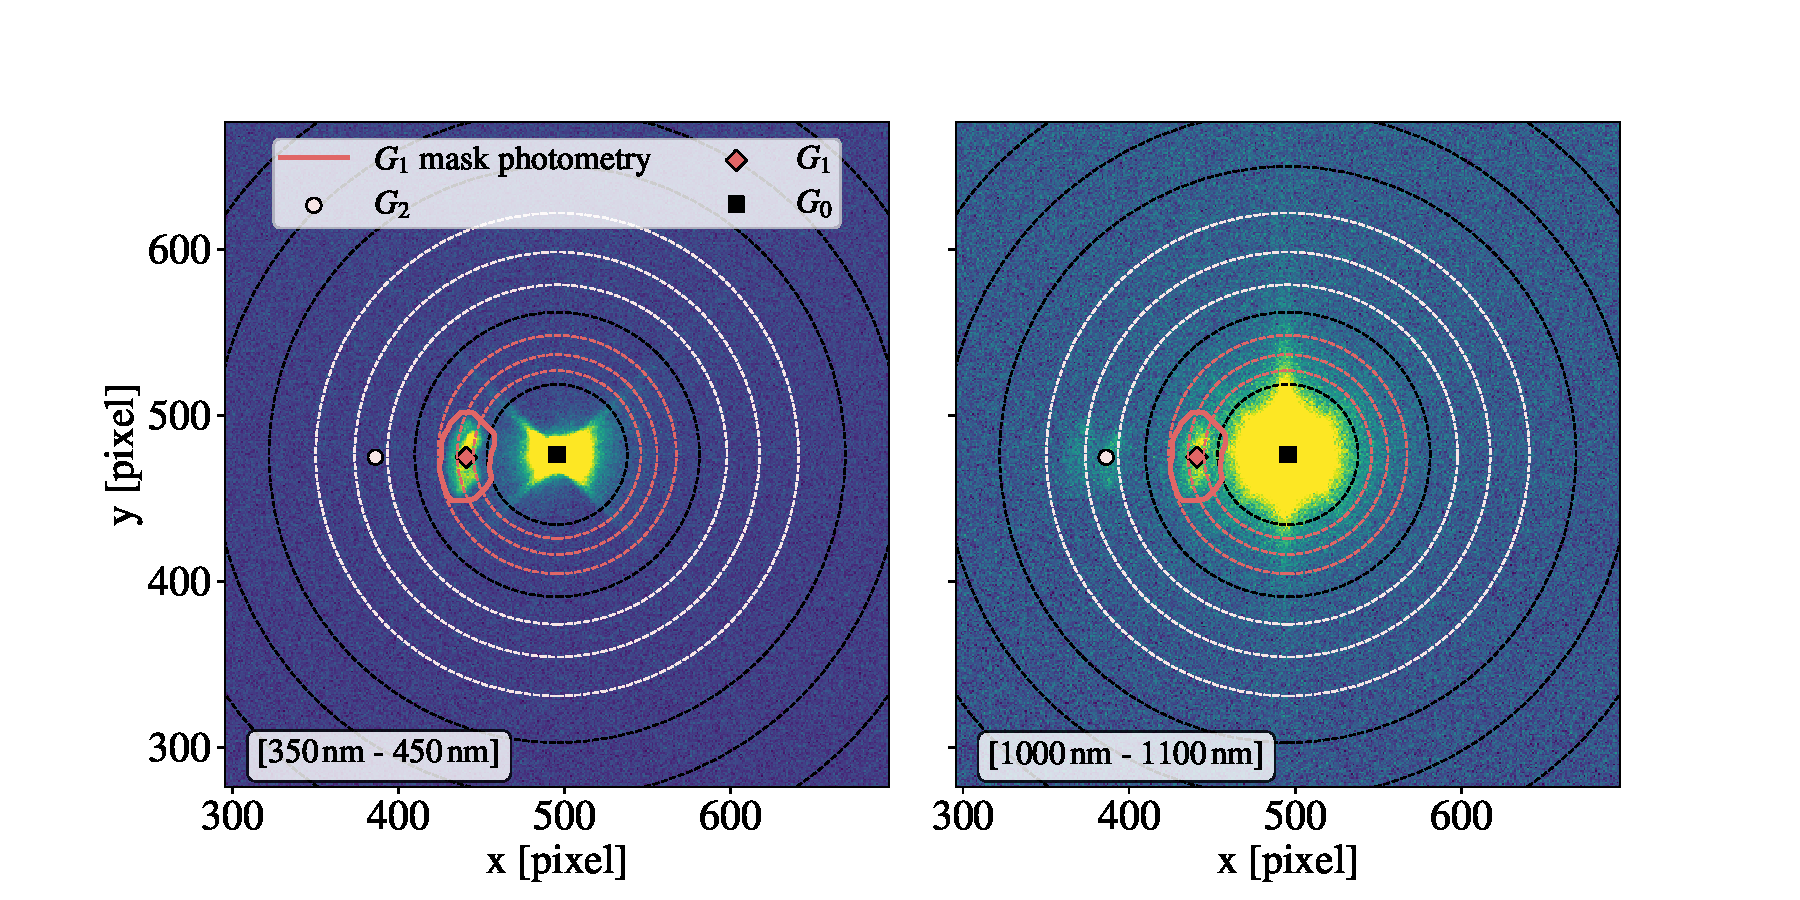
\includegraphics[width=\columnwidth]{fig/ghost_contrast.pdf}
    \caption{Stack of images at different wavelengths, with one image per nanometer. \textit{Left:} Stack of images between \SI{350}{\nano\meter} and \SI{450}{\nano\meter}. The scale is set on the ZScale from IRAF to make faint features visible. The spot of interest $G_0$ is at the center, and the ghost reflections are at its left. The circles correspond to the aperture photometry at different radii, when an annulus contains ghost contribution, it is colored with respect to the order of the ghost. The red area around the 1$\up{st}$ order ghost represents the area where the photometry of the ghost is measured. \textit{Right:} Same image but for a stack of images between \SI{1000}{\nano\meter} and \SI{1100}{\nano\meter}. We note that the 2$\up{nd}$ order ghost is not visible for the stack in the UV, where the 1$\up{st}$ order is maximal, while it is visible in the IR, where the 1$\up{st}$ order is lower. For the stack in IR, we osberve a degradation of the \SD PSF.}
    \label{fig:ghost_contrast}
    %~/stardice/analysis/cbp_paper/total_fluxes/ghost_stack_figure.ipynb
\end{figure}

In this section, we develop a modelization of the \spinhole pinhole dataset, where Figure~\ref{fig:ghost_contrast} shows stacks of images obtained with this dataset. The illumination of a section of the primary StarDICE mirror results in a central image resulting from the \SD telescope PSF, and a set of additional fainter images that we call ghosts. The ghosts result from undesired but unavoidable reflexions on optical surfaces. The most visible ones come from the beam reflexion on the CCD surface and back reflexion on its covering window, as described in Figure~\ref{fig:schema_ghost}.\\

We consider that the \SD telescope PSF can be modelized as a Moffat distribution \citep{moffat} $M(r, \lambda)$ which depends on the radius $r$ and the wavelength $\lambda$ as:

\begin{equation}
M(r, \lambda)= 1 - \left( 1+\frac{r^2}{\alpha(\lambda)^2} \right)^{1-\beta(\lambda)},
\end{equation}
with $\alpha(\lambda)$ and $\beta(\lambda)$ the parameters of the Moffat distribution. The flux $F(r, \lambda)$ measured in the CCD with aperture photometry, can be modelized as: 

%Thus, the core of the spot in the CCD is the convolution of the PSF, the CBP output shape, and ghosts from light reflections between the glass before the CCD and the CCD itself, as schematized in Figure~\ref{fig:schema_ghost}. These contributions make the core of the spot complex to model. However the tail of the PSF should not be impacted by the contribution of the CBP output shape and the light diffusion, so it is expected to behave like a Moffat distribution. 

\begin{equation}
F(r, \lambda) = A(\lambda) \times \frac{M(r, \lambda) + \Kghostfit(r, \lambda)}{1 + \Kghostfit(r \rightarrow +\infty, \lambda)} + \bkg(r, \lambda),
\label{eq:moffat_model}
\end{equation}
with $A(\lambda)$ the total amplitude, $\Kghostfit(r, \lambda) = \frac{\sum_{n=1}^{+\infty} G_n(\lambda)}{A(\lambda)}$ the relative contribution of the sum of all the ghosts $G_n(\lambda)$ and $\bkg(r, \lambda)$ the contribution of the background. The origin of the ghost contribution is schematized in Figure~\ref{fig:schema_ghost}.

The fit is done with PSF photometry for a radius $r=\SI{20.9}{pixels}$, and then for successive annulus of external radius from \SI{24.9}{pixels} to \SI{419.1}{pixels}. These radii are regularly spaced on a logarithm scale shown in Figure~\ref{fig:ghost_contrast}. The parameters of the fit are adjusted with the \spinhole pinhole dataset No.~8 from Table~\ref{tab:schedule}, with one image per wavelength. To take into account $\Kghostfit(r, \lambda)$, an additive value is fitted for every annulus that contains a ghost contribution. The evolution of the Moffat distribution is expected to be smooth with respect to wavelength, so the parameters $\alpha(\lambda)$ and $\beta(\lambda)$ are developed on a B-spline basis with 15 wavelength nodes regularly spaced between \SI{350}{\nano\meter} to \SI{1100}{\nano\meter}. The same goes for the function $\Kghostfit(r, \lambda)$ as it corresponds to light reflections on surfaces in the optical path. The results of this fit are shown Figure~\ref{fig:result_params}. 

\begin{figure}[h]
    \centering
    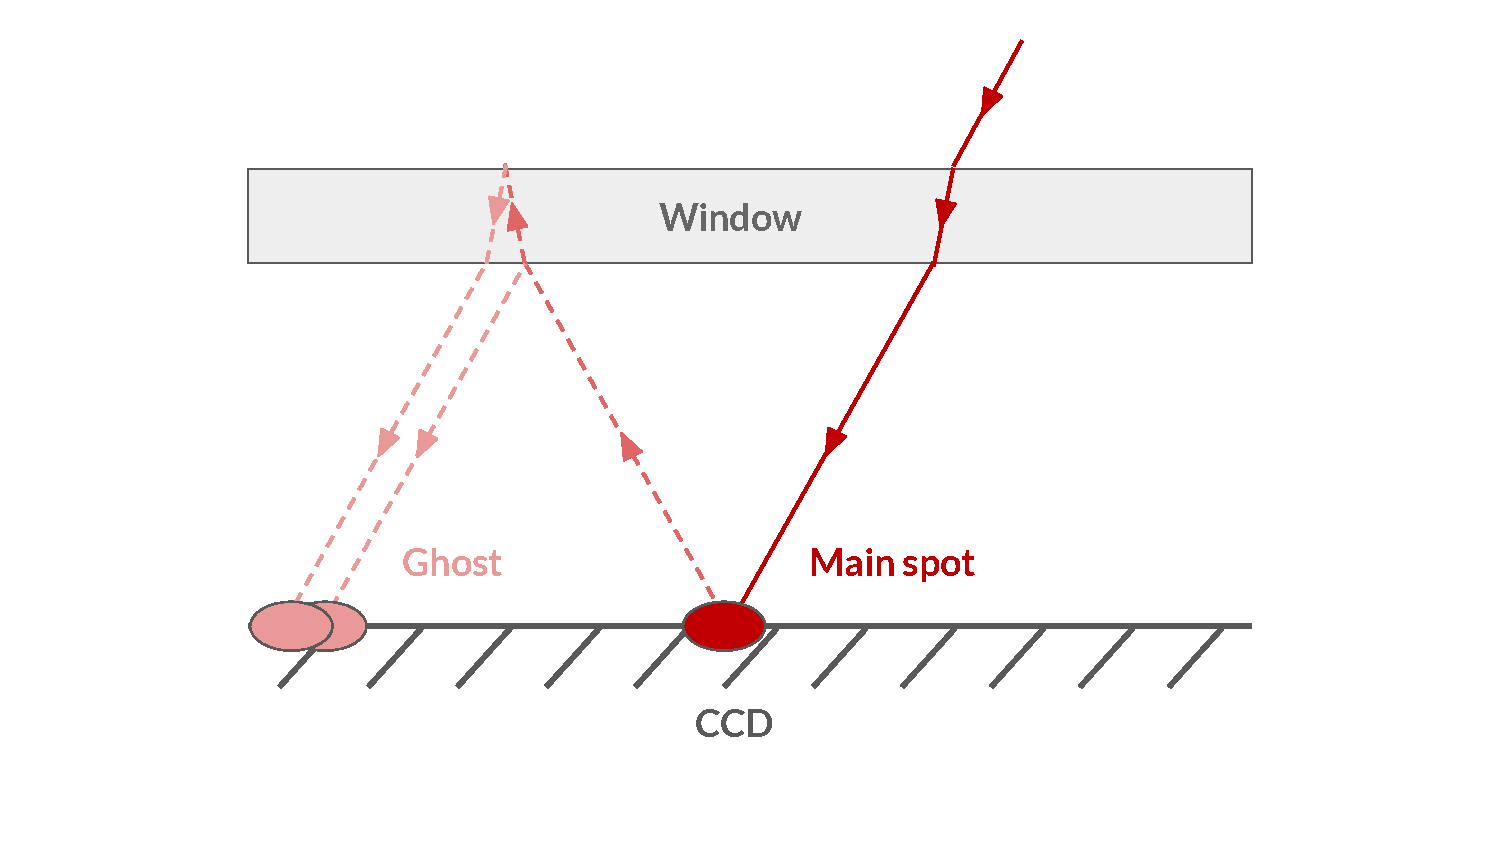
\includegraphics[width=\columnwidth]{fig/schema_ghost.pdf}
    \caption{Schematic of the light reflections that generate the ghosts, which are defocused and less intense images at other positions in the focal plane. A fraction of the light is reflected at the different interfaces and $G_0(\lambda)$, $G_1(\lambda)$ and $G_2(\lambda)$ are respectively the main spot, the 1\up{st} order ghost, and the 2\up{nd} order ghost.}
    \label{fig:schema_ghost}
    %Google slides
\end{figure}

In the first and second panel, we can see that the $\alpha(\lambda)$ and $\beta(\lambda)$ parameters of the PSF are stable within \SI{350}{\nano\meter} and \SI{900}{\nano\meter}, and change significantly beyond. This is correlated with a change of the PSF shape in the infrared as can be seen in the image stacks in Figure~\ref{fig:ghost_contrast}. 

The third panel shows a constant background against wavelength, with a mean of $\mu_\mathrm{bkg, fitted}=\SI{0.267}{ADU/pixel}$ for an exposure time of \SI{1.1}{\second}. This panel show also the result of an independant study of the background analyzing dark images. Two datasets of dark images have been studied, one with the laser turned off, and a second by masking the CBP output with a cap (dataset No.~9 in Table~\ref{tab:schedule}). Both datasets are constants in time and wavelength, and their mean value of ADU/pixel are compatible, so we combine them into one dataset of darks. The mean photometry value of this dataset is represented by the black dashed line in this third panel, and is $\mu_\mathrm{dark, photometry}=\SI{0.252}{ADU/pixel}$ with a standard deviation $\sigma_\mathrm{dark, photometry}=\SI{0.059}{ADU/pixel}$. We conclude that the estimation of the background with the fit is consistent with the dark datasets results. \\

The fourth panel presents the relative contribution of the first order ghost $G_1(\lambda)$, $\Kghostfitfirst(\lambda) = \frac{G_1(\lambda)}{A(\lambda)}$ in percent, superimposed with the fraction $\Kghost=\frac{G_1(\lambda)}{G_0(\lambda)}$ obtained by photometry measurements on the first order ghost $G_1(\lambda)$ and the main spot $G_0(\lambda)$. The method to perform ghost photometry is detailed in Appendix~\ref{sec:ghost_photometry}. The ratio $\Kghost$ and $\Kghostfitfirst$ obtained with two different methods on two different datasets are superimposing well below \SI{950}{\nano\meter}, which gives us confidence about the accuracy of this measurement. The deviation above \SI{950}{\nano\meter} between the two methods can be explained by the following arguments. the $\alpha(\lambda)$ and $\beta(\lambda)$ parameters indicate a deterioration of the PSF, which starts to overflow in the ghost photometry. In addition, interference fringes are appearing in the focal plane at these wavelengths, complicating the ghost photometry. As the fit accounts for the PSF evolution, the fitted result gives more confidence in its accuracy.

The reduced chi-squared of the fit in the fifth panel reach a value close to 1 at every wavelength, which indicates that the model satisfactorily describes the dataset.

\begin{figure}[h]
     \centering
     \resizebox{\hsize}{!}{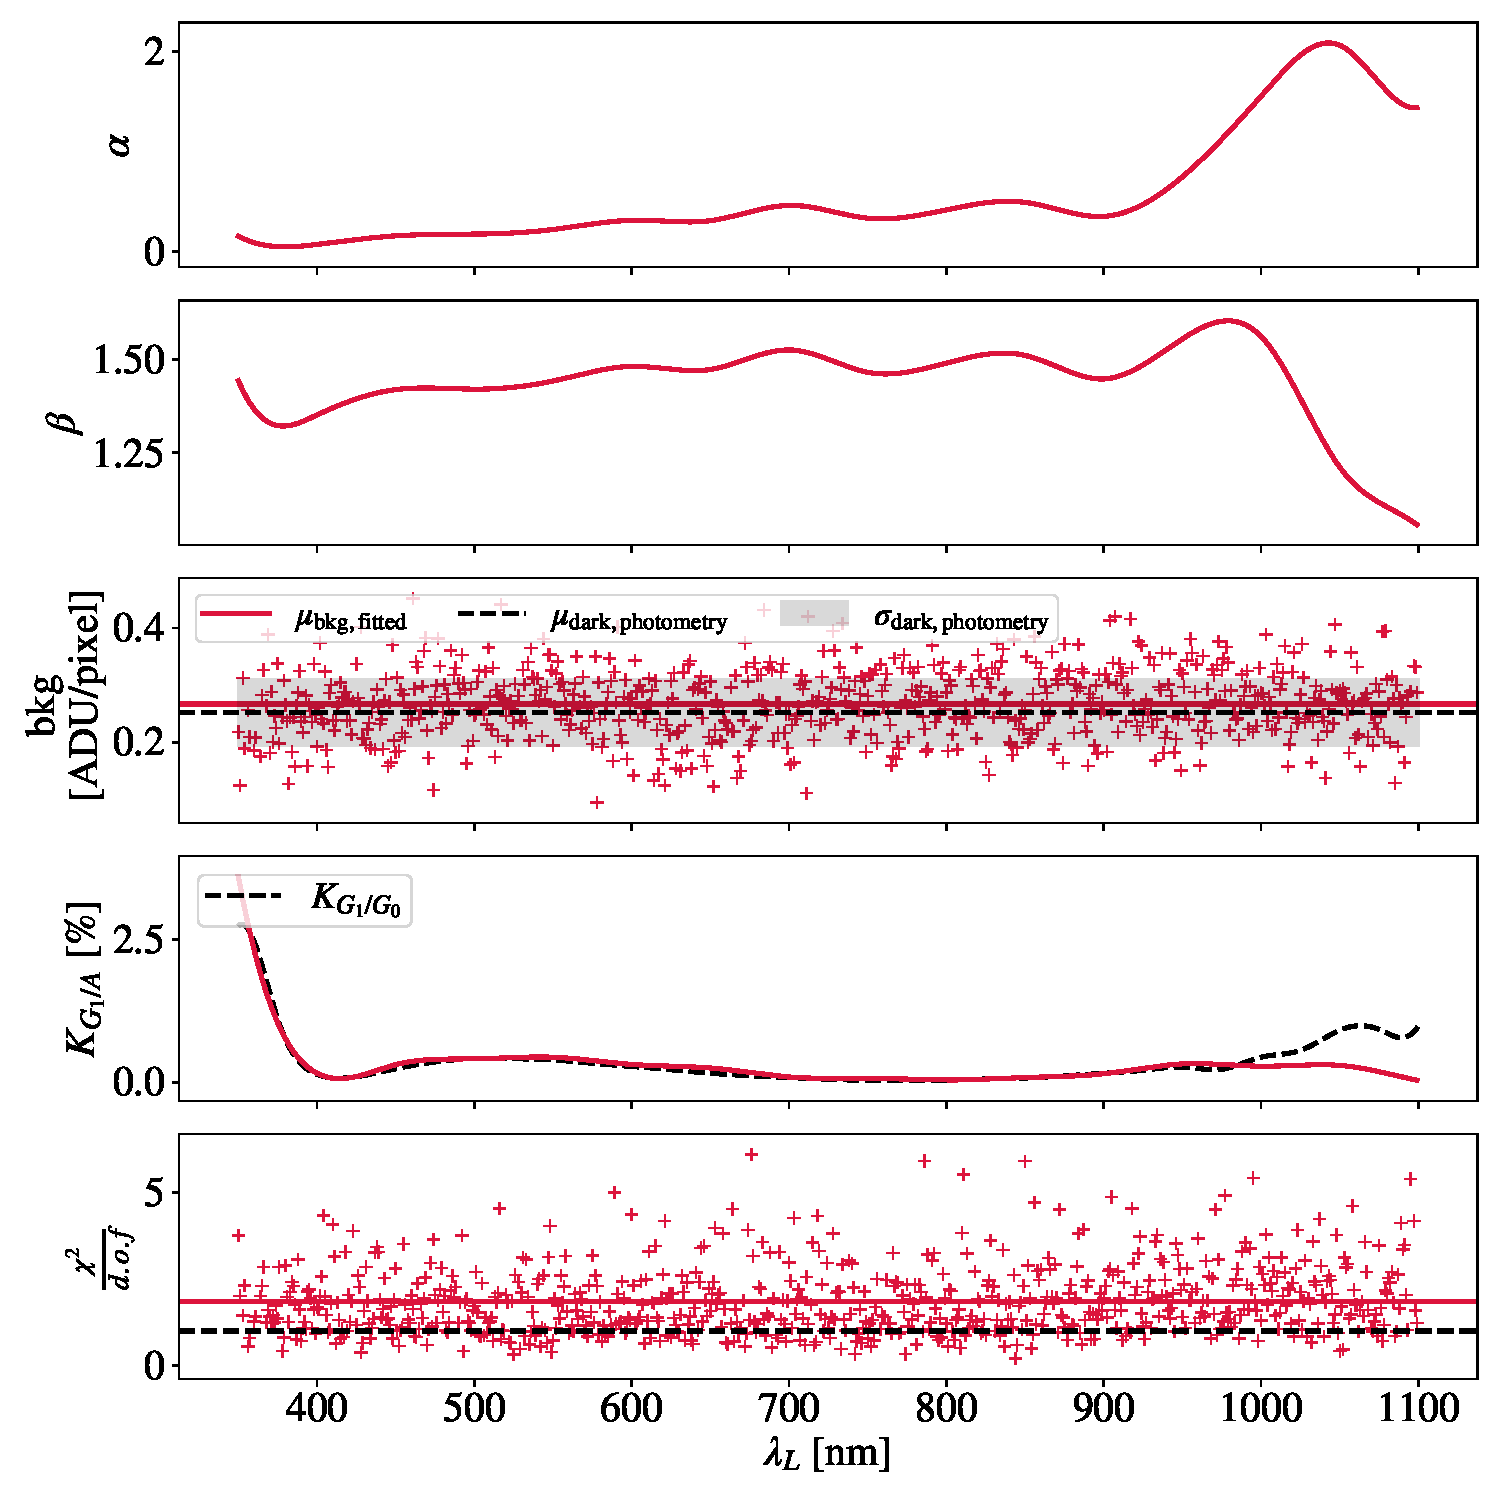
\includegraphics{fig/result_params.pdf}}
     \caption{Best fitting parameters for the model of Equation~\ref{eq:moffat_model}. Red plain lines correspond to the result of the fit, and black dashed lines to the values expected. From top to bottom: the first and second panel represent respectively the $\alpha(\lambda)$ and $\beta(\lambda)$ parameters from the Moffat distribution; the third panel shows the background contribution per pixel and its mean value in red, while the dark dashed line is the mean value of the dark; the fourth panel represents $\Kghostfitfirst(\lambda)$, and $\Kghost$; the fifth panel represents the reduced chi-squared of the fit.}
     \label{fig:result_params}
    %~/stardice/analysis/cbp_paper/total_fluxes/fit_results.ipynb
\end{figure}

%II. photométrie portable sur ciel 
%
%on peut modéliser pcq on n'a pas de fond --> propre aux images CBP (pas de fond ciel, source isolée), donc peut pas faire en pratique sur ciel
%
%comme d'hab : soustraction de fond classique et se limiter à ouverture donnée ~20 pixels
%si on fait ça, voilà la fraction du flux qu'on récupère : plot de correction d'ouverture phi20/A (quantifier les biais sur F(20)/A et ap_bkg ou fit_bkg), biais à cause du flux perdu et biais à cause de la source  
%
%Problèmes IR:
%1) params fitté partent aux fraises dans l'IR, ça doit venir de StarDICE, peut-être transparence du télescope (regarder dans le filtre y comparé au filtre g ou i) --> peut pas reconstruire de manière précise le flux d'une étoile au-delà de 1000nm (pas de lien entre CBP et obs stardice)
%
%On va mesurer l'ensemble des spots CBP avec l'ouverture à 20 pixels sachant que dans l'IR c'est pas fou 
%*98\% du flux stable en couleur

\subsection{Photometry for filter throughput measurement}
\label{sec:photometry_small}

The modelization of the PSF at long distance from its core is possible because of the laboratory conditions of these images. These conditions are intrisinc to CBP images, with an isolated source and no sky background. It is impossible to port this method with on-sky data. We choose to carry out the whole analysis with aperture photometry and a background estimation reproducible with on-sky data. This method is the baseline photometry for the \spinhole pinhole, and we compared the measurements obtained with such a method and the fitted parameters to quantify eventual biases. 

\subsubsection{Background subtraction}
\label{sec:bkg}

To estimate the background contribution, the sources in the image need to be detected and masked. We compute the standard deviation of an image $\sigma$, and every pixel with a signal higher than 5$\sigma$ is masked, as well as all the surrounding pixels that has a signal higher than 2$\sigma$. Then we proceed to a segmentation of the masked image into boxes of $129\times132$ pixels. We compute the mean and the standard deviation of the background in each of these boxes, and we interpolate their values in a 2D map to get our estimation of the background. This background estimation is subtracted to the image. Then, the centroid of the spot of interest is computed to pursue aperture photometry at this position. $\Qccd$ is measured with aperture photometry at a radius of \SI{20.9}{pixels} for every image of the dataset with the \spinhole.

\subsubsection{Correction of the light contamination}\label{sec:sd_contaminations}

When measuring the flux collected from the \SD camera, we have to remove light contaminations described in Sections~\ref{sec:532_cont} and~\ref{sec:fluorescence}. As the photodiode and the solar cell, the total signal measured in the \SD camera $\Qccdmes$ is the sum of the flux from the main laser line $\Qccdcal$ and the flux from the \SI{532}{\nm} contamination $\Qccd^{532}$, the $\lambda_{\rm comp}$ contamination $\Qccd^{\lambda_{\rm comp}}$, and the integrating sphere fluorescence $\Qccd^{\mathrm{fluo}}$, as follows:
\begin{equation}
    \Qccdmes = \Qccdcal + \Qccd^{532} + \Qccd^{\lambda_{\rm comp}} + \Qccd^{\mathrm{fluo}}
    \label{eq:qccd_mes}
\end{equation}

The contamination light in the \SD camera can be estimated by multiplying $\Qphot^{532}$, $\Qphot^{\lambda_{\rm comp}}$ and $\Qphot^{\mathrm{fluo}}$ by $\Rcbp(\lambda)$ and $\Rtel(\lambda)$. The contaminations are subtracted, and impact on filter transmission measurement is shown Figure~\ref{fig:g_filter_532}, focusing on the \SD g filter, the most affected filter by integrating sphere fluorescence and \SI{532}{\nano\meter} line.

\begin{figure}[h]
    \centering
    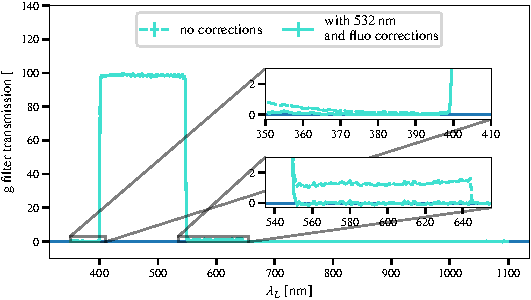
\includegraphics[width=\columnwidth]{fig/g_filter_532.pdf}
    \caption{\SD g filter transmission as a function of the set laser wavelength $\lambda_L$, with and without the \SI{532}{\nm} and fluorescence correction. For clarity, we added a zoom on the out-of-band transmission where $\SI{532}{\nm}$ line is transmitted while higher wavelengths are shot by the laser.}
    \label{fig:g_filter_532}
    %cbp_paper_plots.ipynb
\end{figure}

\subsubsection{Aperture correction}

In this section, we aim to quantify the fraction of flux missed when measuring the signal for a \spinhole pinhole image with aperture photometry rather than with the PSF photometry. We define the faction of flux missed as the ratio between the value measured with photometry for a given radius and the total amplitude $A$ fitted for a given wavelength. It is quantified in Figure~\ref{fig:bias_aperture}. Less than 3\% of the flux is missed between \SI{400}{\nano\meter} and \SI{900}{\nano\meter}. Below \SI{400}{\nano\meter} the ghost contribution is missed when using an aperture of \SI{20.9}{pixels}. Above \SI{900}{\nano\meter} where the PSF is degrading, the fraction of flux missed increase by one order of magnitude and reach more than 75\%. The bottom panel of Figure~\ref{fig:bias_aperture} shows that the baseline photometry is compatible to the fit estimation at less than 0.2\% between \SI{400}{\nano\meter} and \SI{900}{\nano\meter}. 

\begin{figure}[h]
     \centering
     \resizebox{\hsize}{!}{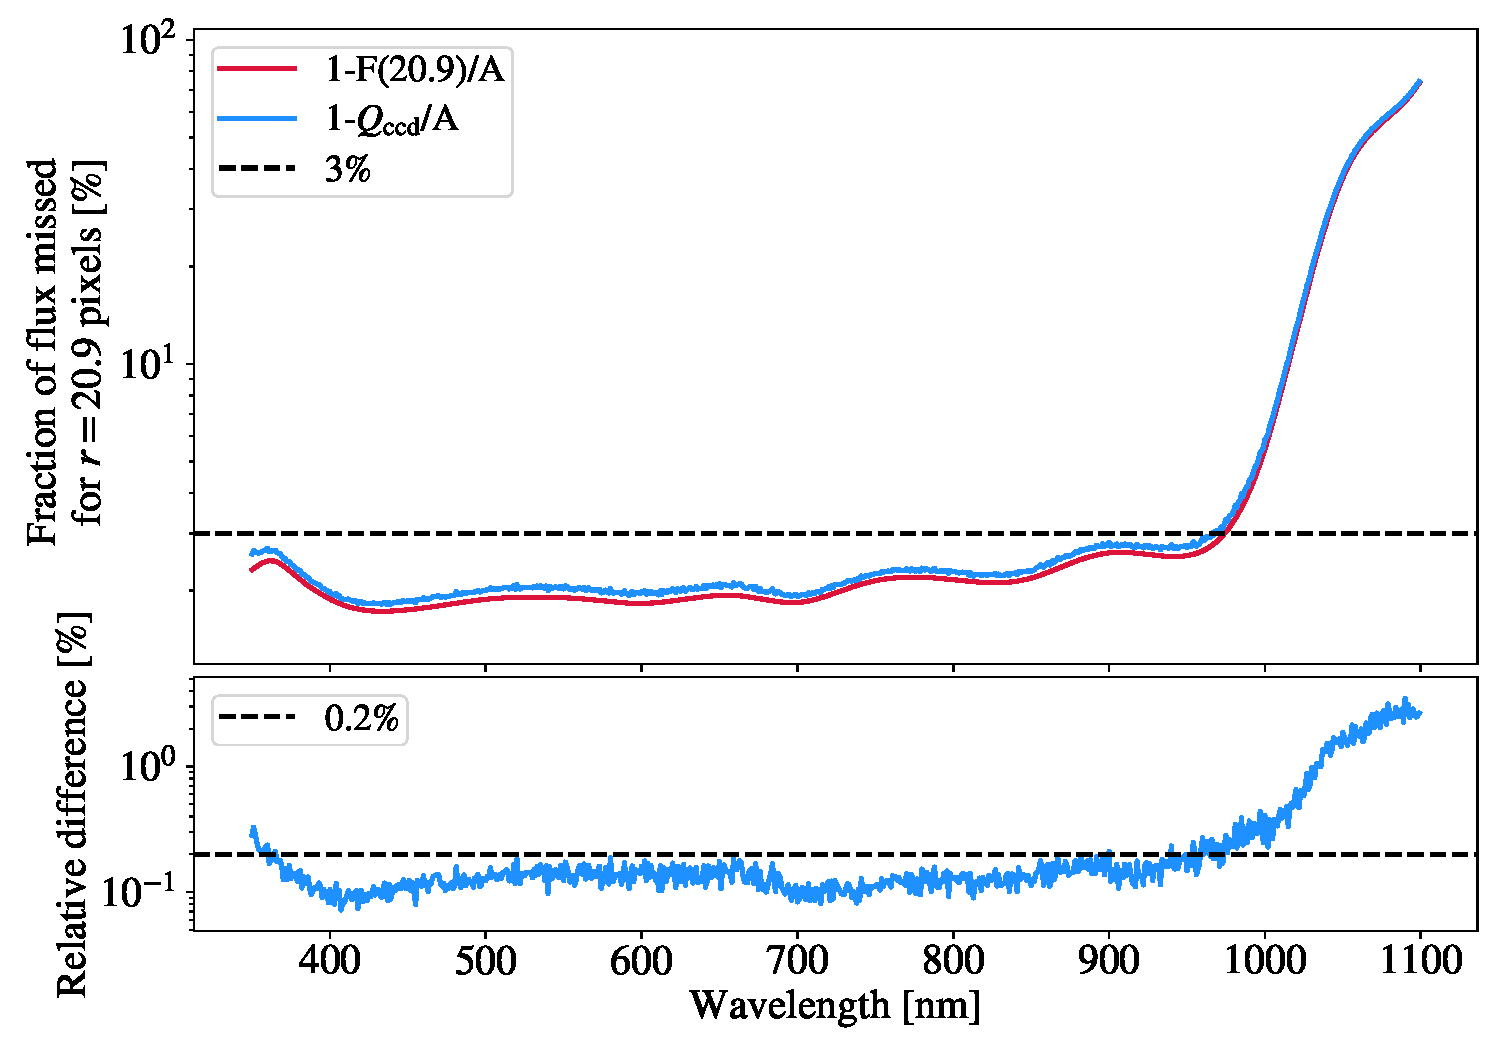
\includegraphics{fig/bias_aperture.pdf}}
     \caption{\textit{Top:} Fraction of missing flux against $\lambda_L$ when measuring \spinhole pinhole dataset with aperture photometry at \SI{20.9}{pixels} rather than taking the total amplitude $A$ fitted. The red curve corresponds to the estimation of the fit, the green one to aperture photometry when the backgruond is estimate with the dark datasets, and the blue one to aperture photometry when the background is estimate with the method described in Section~\ref{sec:photometry_small}. \textit{Bottom:} Relative difference in percent between the flux measured for aperture photometry with the two background estimations and the model estimation at \SI{20.9}{pixels}.}
     \label{fig:bias_aperture}
    %~/stardice/analysis/cbp_paper/total_fluxes/fit_results.ipynb
\end{figure}

We can reach the conclusion that the baseline aperture photometry for the \spinhole pinhole can be used for the range between \SI{400}{\nano\meter} and \SI{900}{\nano\meter}. Below \SI{400}{\nano\meter} there is a need to take care of the ghost contribution. Above \SI{900}{\nano\meter}, this method does not measure a representative flux of the target. It is believed that the \SD telescope is the one responsible for the PSF degradation, one possible explanation is that the primary mirror is becoming partially transparent and generate defocused light. Anyhow, the CBP measurements cannot be trusted in this wavelength range. 

\subsubsection{Pinhole intercalibration}

It is necessary to intercalibrate the \SD response measurements obtained with the \spinhole pinhole with the CBP response measurements obtained with the \bpinhole pinhole. To link these measurements, we measure the \SD responses with the \spinhole pinhole and the \bpinhole pinhole and compute the pinholes ratio $\Kpinholes$. This ratio is defined such as the $\Rcbp$ defined in Equation~\ref{eq:rsd} is the \spinhole pinhole CBP response $\Rcbp^{\spinhole}$, which can be obtained with the \bpinhole pinhole CBP response $\Rcbp^{\bpinhole}$:

\begin{equation}
	\Rcbp(\lambda) \equiv \Rcbp^{\spinhole}(\lambda) = \Rcbp^{\bpinhole}(\lambda) \times \Kpinholes
\end{equation}

When shooting with the \bpinhole pinhole, the main spot is not a pointlike source, hence the data reduction of $\Qccd^{\bpinhole}$ is different than the baseline photometry. The overscan subtraction and the light contamination correction are done with the same method than the \spinhole pinhole, detailed respectively in \ref{sec:overscan} and \ref{sec:sd_contaminations}. However the background subtraction cannot be performed the same way. 

When using \bpinhole pinhole, the main spot takes a significant area of the focal plane, meaning there is not enough background in the image to reconstruct it. The background is measured with dark exposures with the dark datasets mentioned above, and the spatial mean of all these dark images is computed to obtain a master dark. The background contribution is estimated by aperture photometry in the master dark at the same position and same radius than the laser-on images. $\Qccd^{\bpinhole}$ is measured with aperture photometry, after background subtraction. The optimal radius is evaluated at 300 pixels for the \bpinhole pinhole in order to contain the main spot and the 1\up{st} order ghost. We could have increased the radius to contain the iris flux, but it would have added as much noise as the signal gained. 

To compare the \SD responses for both pinhole, we need to measure the fluxes with aperture photometry at the same radius so that it contains the same features, such as the ghost contribution. This way there is no other consideration than the geometry of the pinholes. We estimate the \spinhole pinhole flux $F(300, \lambda)$, $\Qccd^{\bpinhole}$ with the method described in Section~\ref{sec:photometry_big}. We compute the ratio $\Kpinholes=\frac{F(300)}{\Qccd^{\bpinhole}}$ and show the result in Figure~\ref{fig:ratio_pinholes}. The linear fit of this ratio is used to intercalibrate the \bpinhole pinhole $\Rcbp(\lambda)$ obtained and the \spinhole pinhole \SD for every measurements of this analysis.

%The non-null slope and not expected as the ratio between the two pinholes should corresponds only to the ratio of surfaces of illuminated area at the input CBP. We suspect that some light diffusion on the edges of the pinholes or other complex reflections in the setup could give this ratio a chromatic dependance.


\begin{figure}[h]
    \centering
    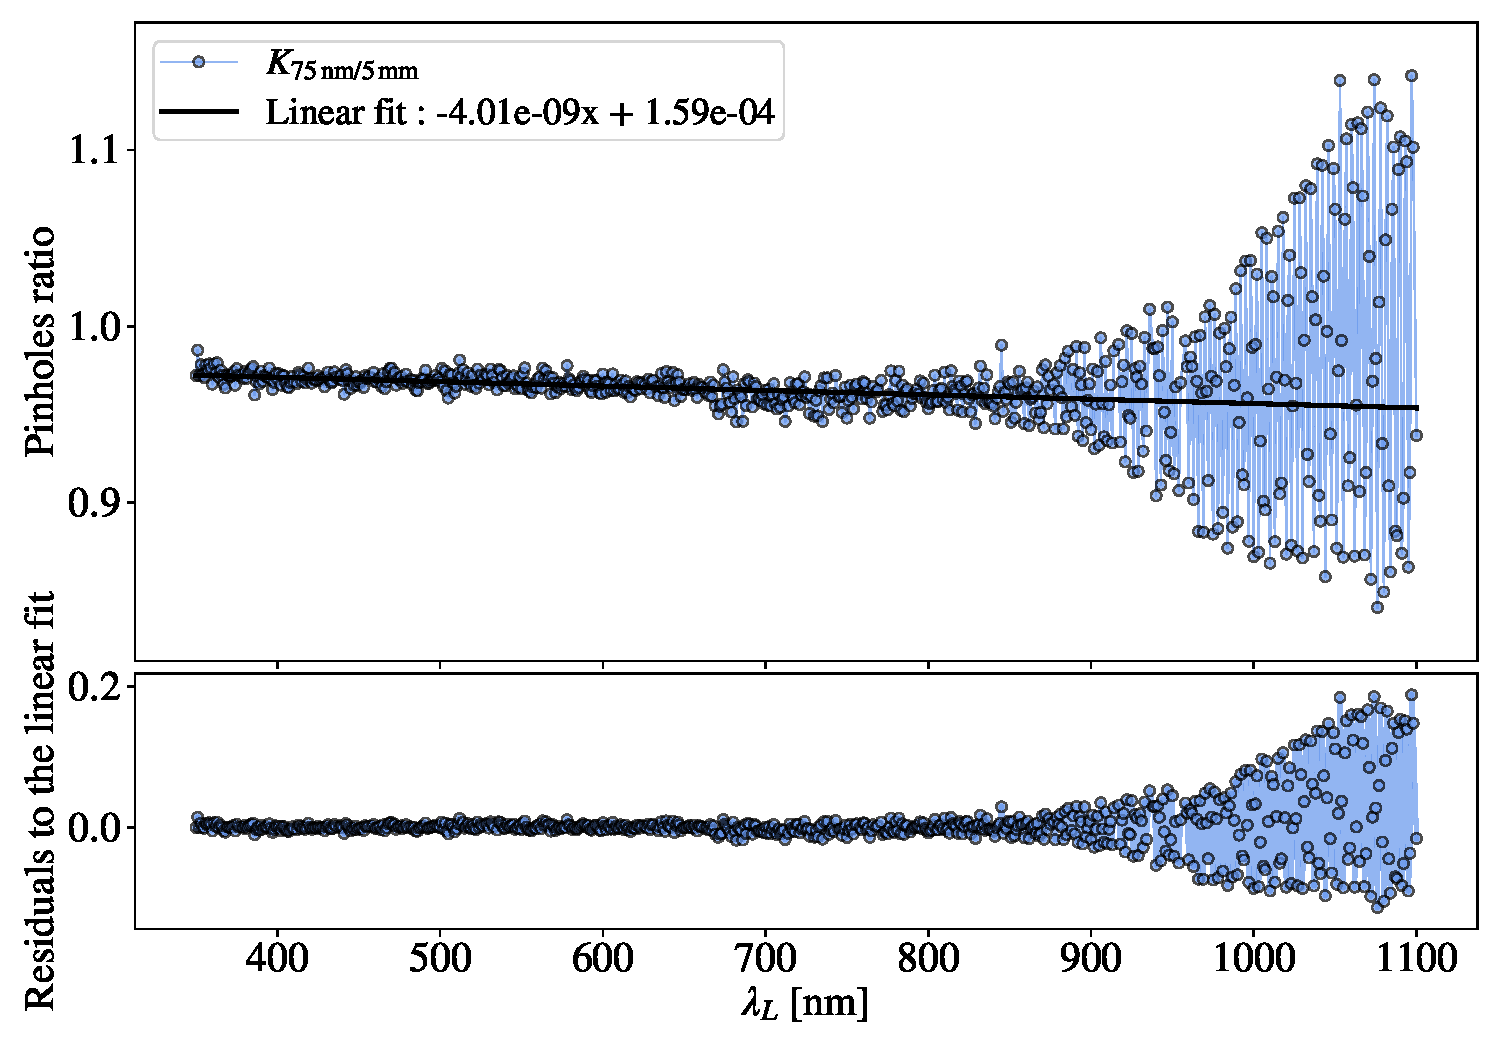
\includegraphics[width=\columnwidth]{fig/ratio_pinholes.pdf}
    \caption{Ratio $\Kpinholes$ with respect to wavelength. The black line corresponds to a linear fit between \SI{400}{\nm} and \SI{900}{\nm}.}
    \label{fig:ratio_pinholes}
    %~/stardice/analysis/cbp_paper/total_fluxes/ratio_pinholes.ipynb
\end{figure}

% The bottom panel corresponds to the aperture correction that is needed to apply to the aperture photometry measurement. It is around 2\% below \SI{950}{\nano\meter}, and increase by one order of magnitude in the infrared. This increase is correlated with the variation of the Moffat parameters $\alpha$ and $\beta$, showing that the PSF is drastically changing in the near infrared. This issue is discussed in more details section \ref{sec:ir}. The third panel show a constant background against wavelength, at a mean of \SI{0.27}{ADU/pixel}.
%
%\subsubsection{Summary}
%
%The summary of the error budget on the \SD telescope response id detailed in Figure~\ref{fig:sd_budget}
%
%
%\begin{figure}
%    \centering
%    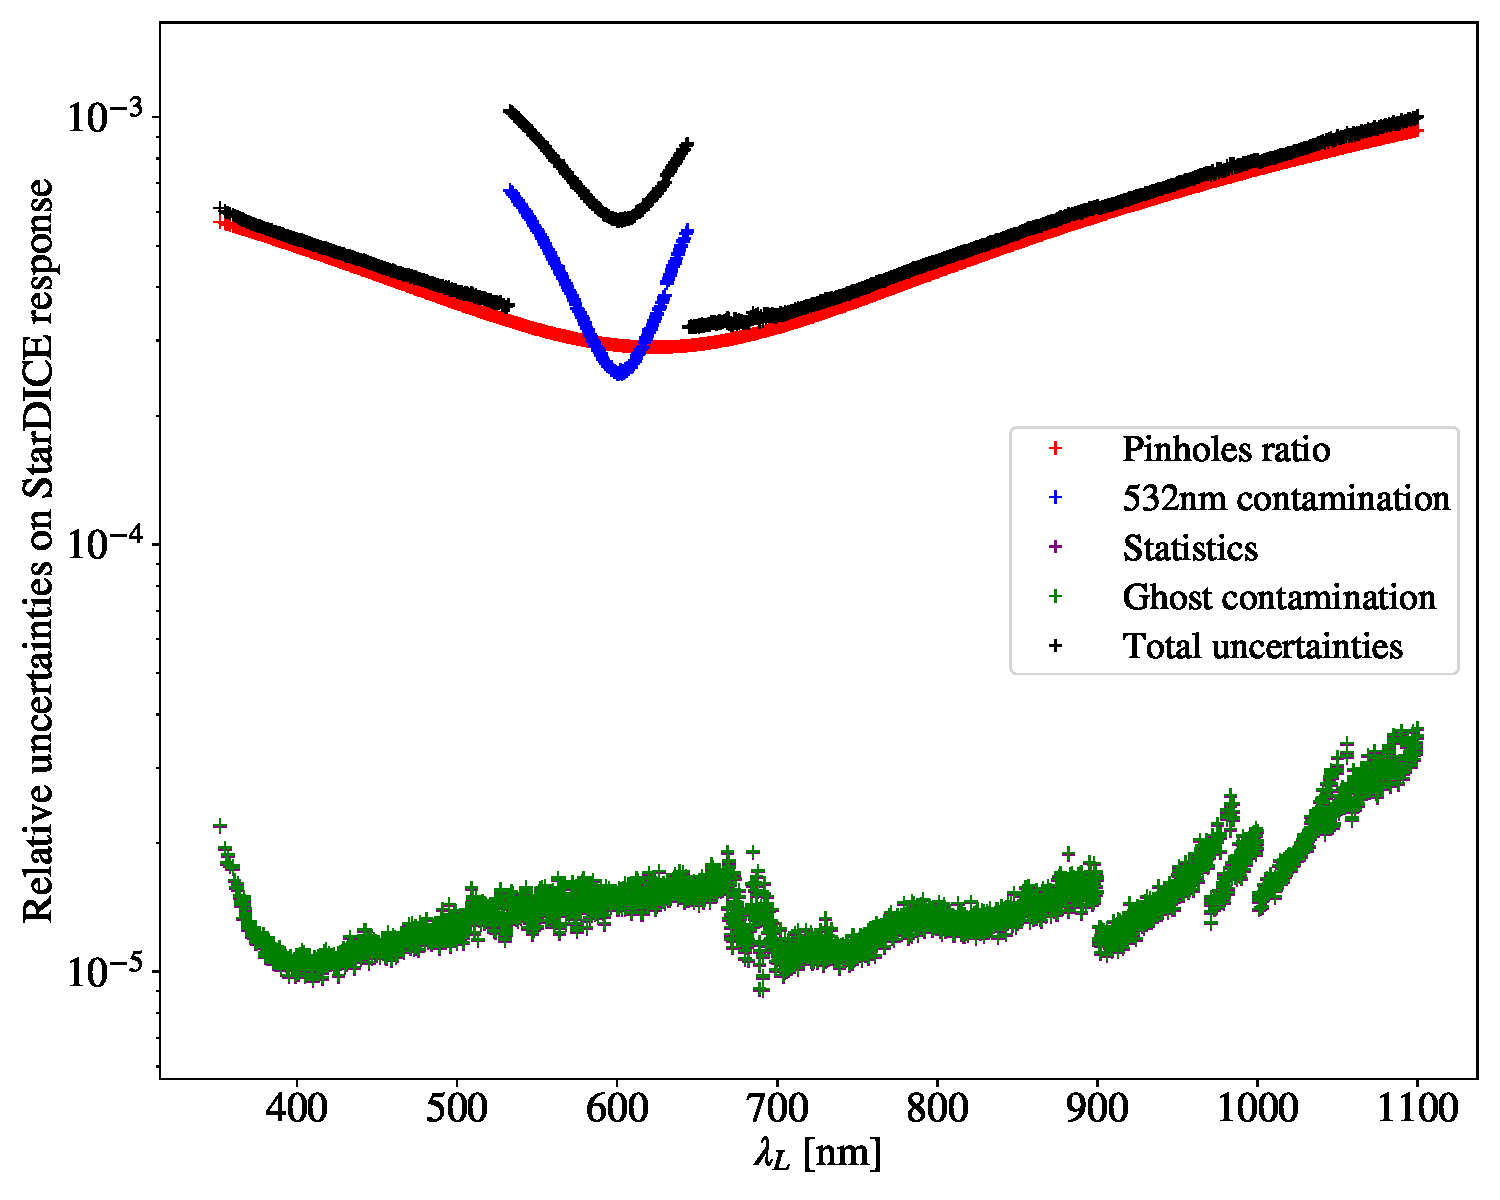
\includegraphics[width=\columnwidth]{fig/sd_uncertainties_budget.pdf}
%    \caption{Total error budget for \SD response.}
%    \label{fig:sd_budget}
%\end{figure}

\subsection{\SD response}

In this section we present the results obtained for the \SD throughput measurement with the \bpinhole pinhole from dataset No.~8; the StarDICE throughput and its filter and grating transmissions measurement with the \spinhole pinhole from dataset No.~6; and the measurements of the datasets No.~2, No.~3 and No.~12. 

\subsubsection{\SD throughput with \bpinhole pinhole}

The Figure~\ref{fig:stardice_5mm_response} show the \SD response obtained with the \bpinhole pinhole, and no filter.

\begin{figure}[h]
    \centering
    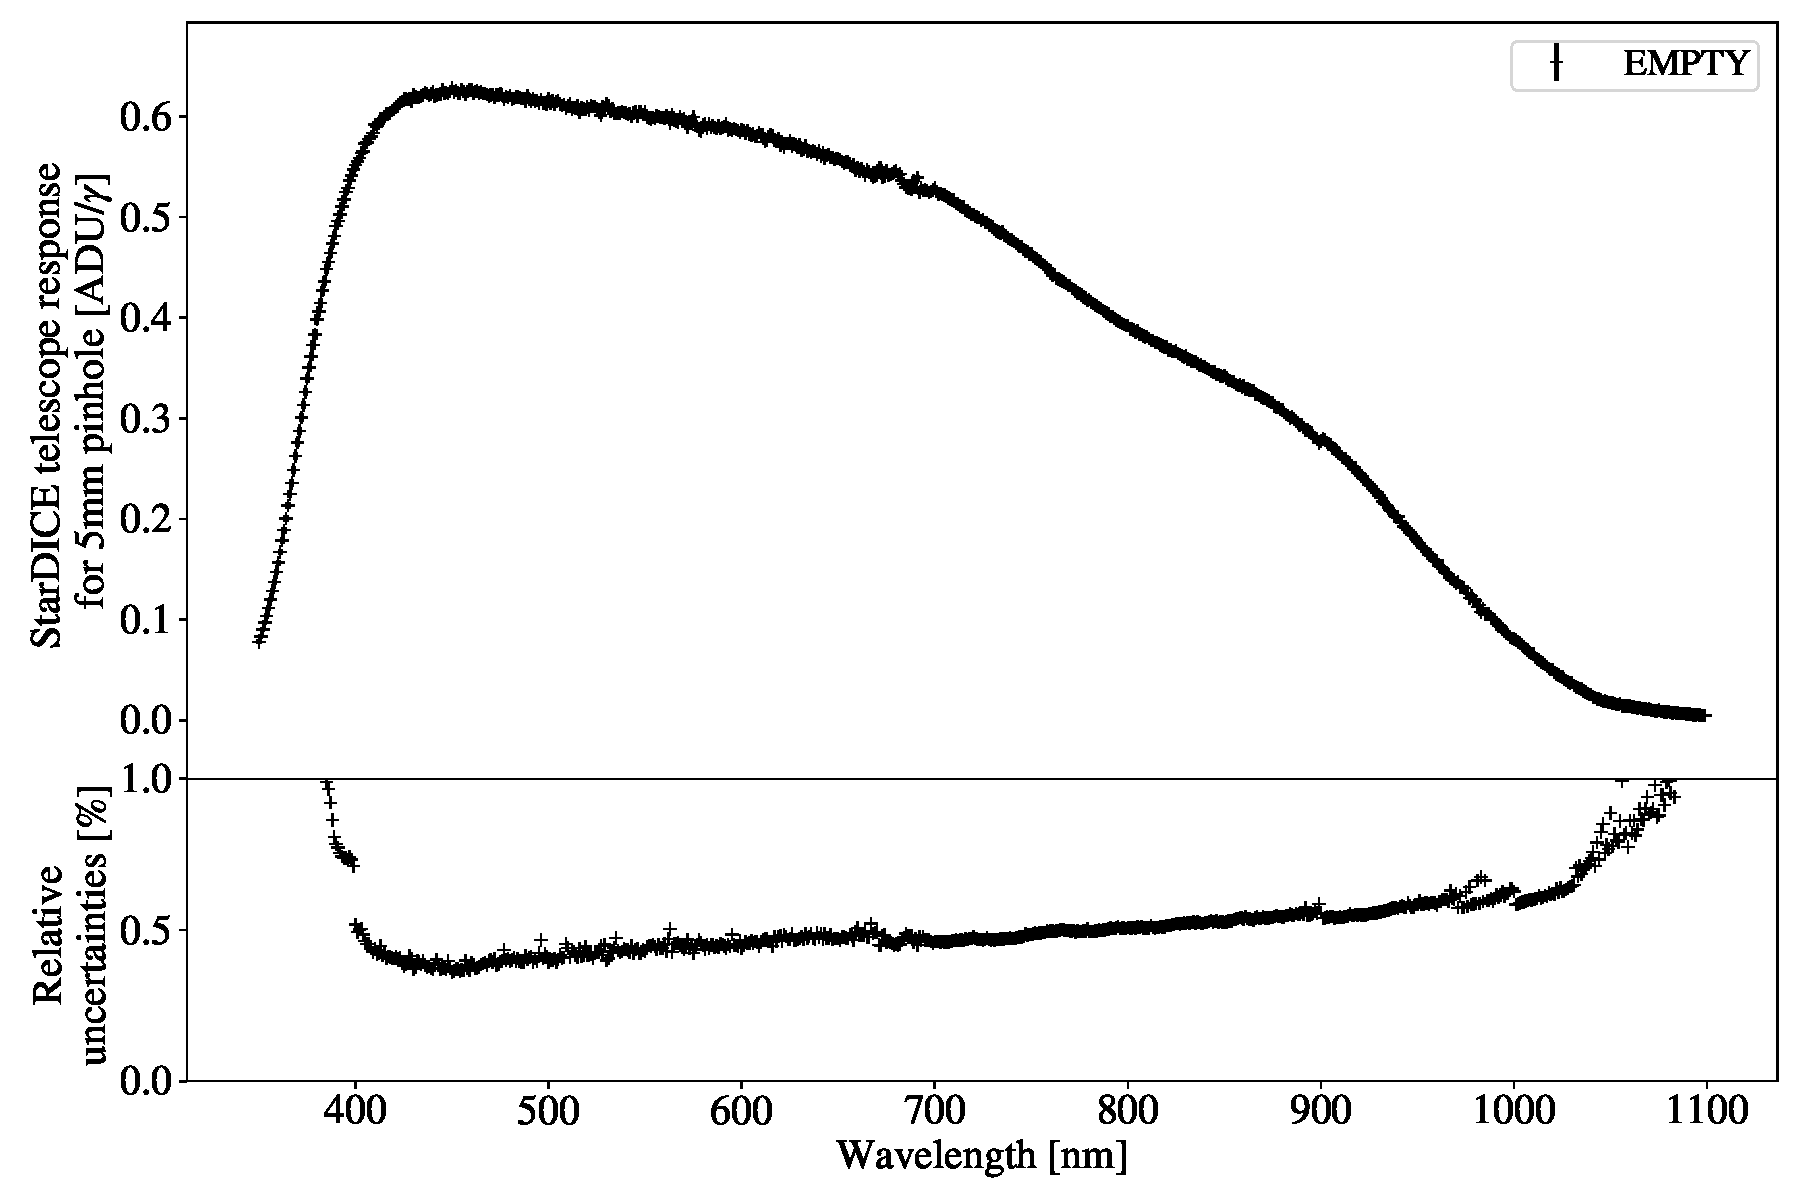
\includegraphics[width=\columnwidth]{fig/stardice_5mm_response.pdf}
    \caption{\textit{Top:} \SD response with no filter and \bpinhole pinhole with respect to wavelength in nanometer. \textit{Bottom:} Uncertainties over the \SD response measurement with respect to wavelength in nanometer.}
    \label{fig:stardice_5mm_response}
    %~/stardice/analysis/cbp_paper/golden_sample_analysis/dr2/response_plots.ipynb
\end{figure}

\subsubsection{\SD throughput and filter transmissions with \spinhole pinhole}

The Figure~\ref{fig:stardice_75um_response} show the \SD response obtained with the \spinhole pinhole, with all filters. In this figure can see that the wavelength resolution is precise enough to have several points in the filter edges, which is a good feature to measure precisely the filter central wavelength. 

\begin{figure}[h]
    \centering
    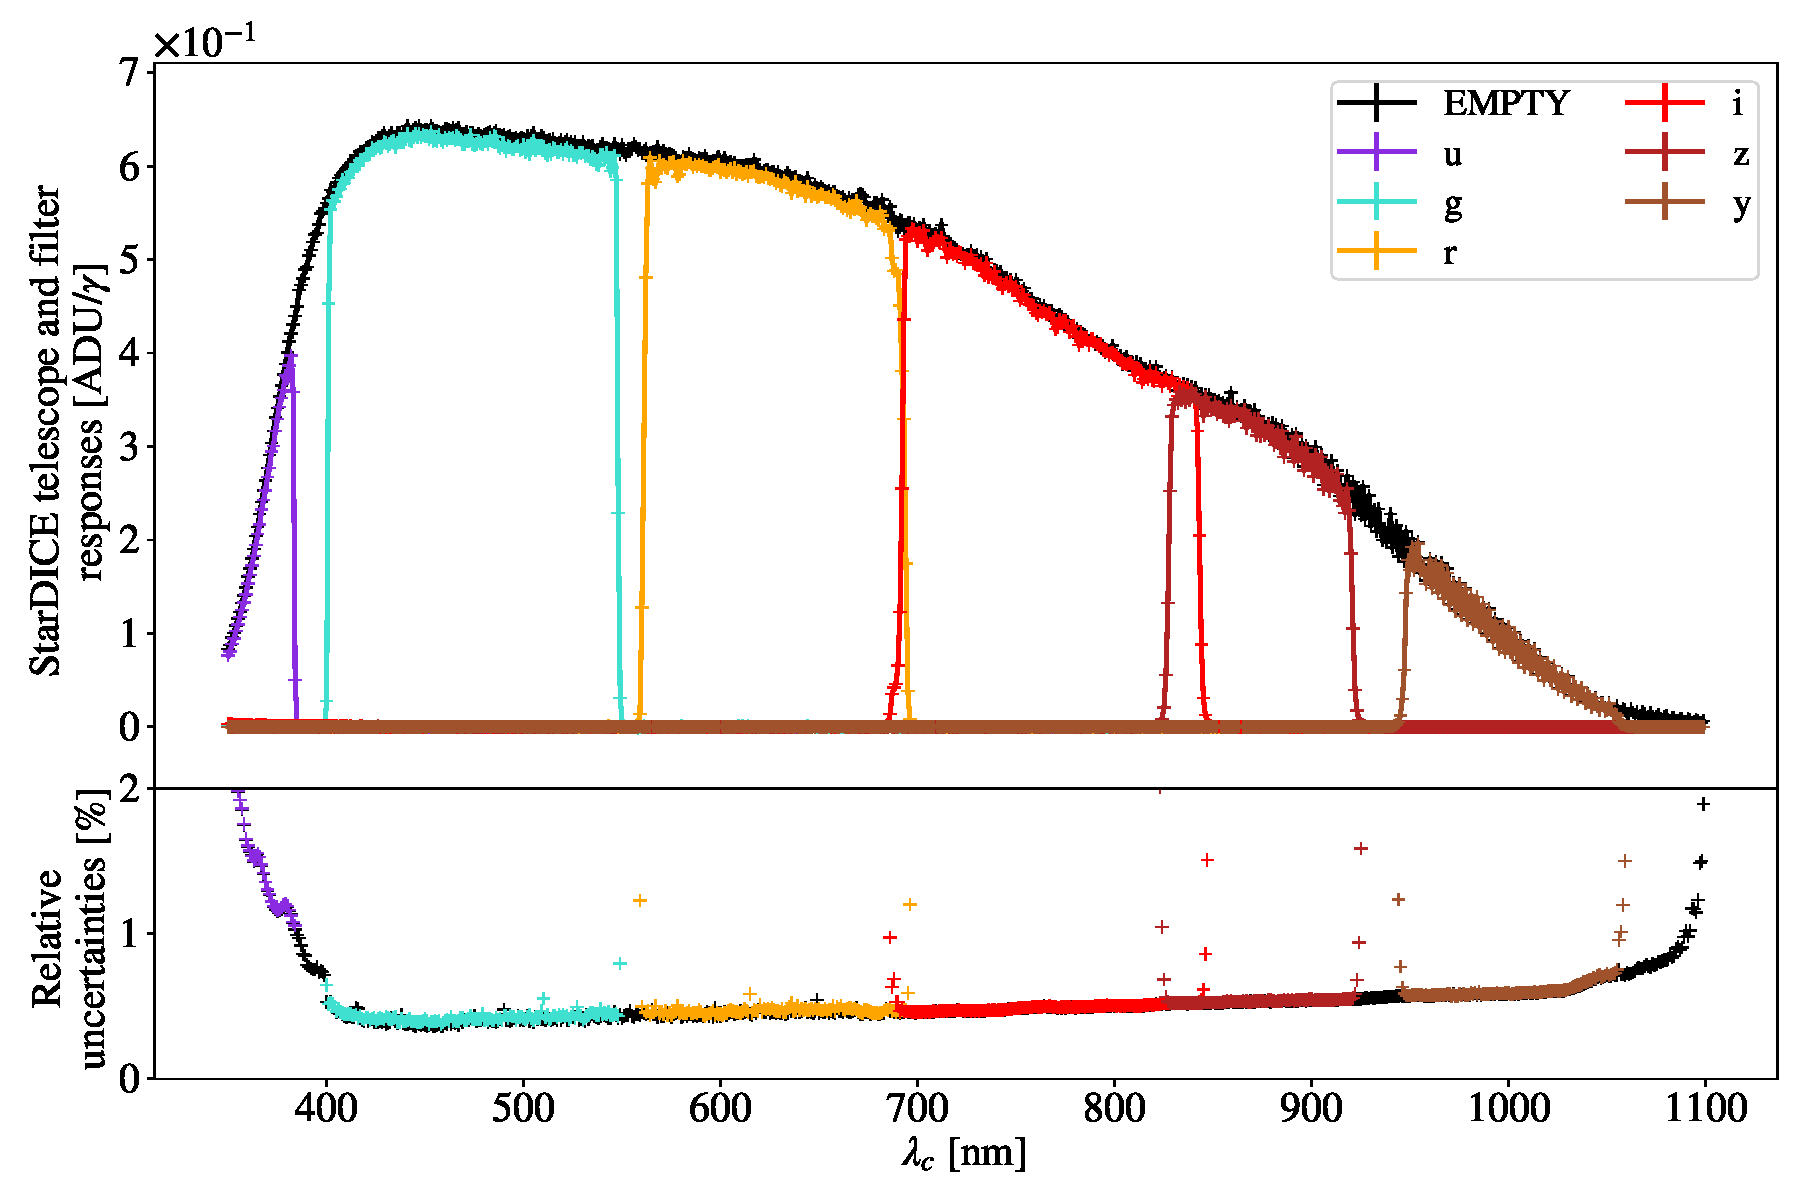
\includegraphics[width=\columnwidth]{fig/stardice_75um_response.pdf}
    \caption{Up : \SD response with at all filters and \spinhole pinhole with respect to wavelength in nanometer. \textit{Bottom:} Uncertainties over the \SD response measurement with respect to wavelength in nanometer.}
    \label{fig:stardice_75um_response}
    %~/stardice/analysis/cbp_paper/golden_sample_analysis/dr2/response_plots.ipynb
\end{figure}

\subsubsection{\SD grating transmissions}

The Figure~\ref{fig:stardice_grating_response} show the \SD response obtained with the \spinhole pinhole, with the grating set in the filterwheel. The grating being blazed so that the 1\up{st} order of diffraction is the brightest, so this is where the signal is the better as it can be seen in the relative uncertainties panel. We see a cut of the 2\up{nd} and 3\up{rd} order that correspond to the wavelength at which the signal is outside the CCD sensor.

\begin{figure}[h]
    \centering
    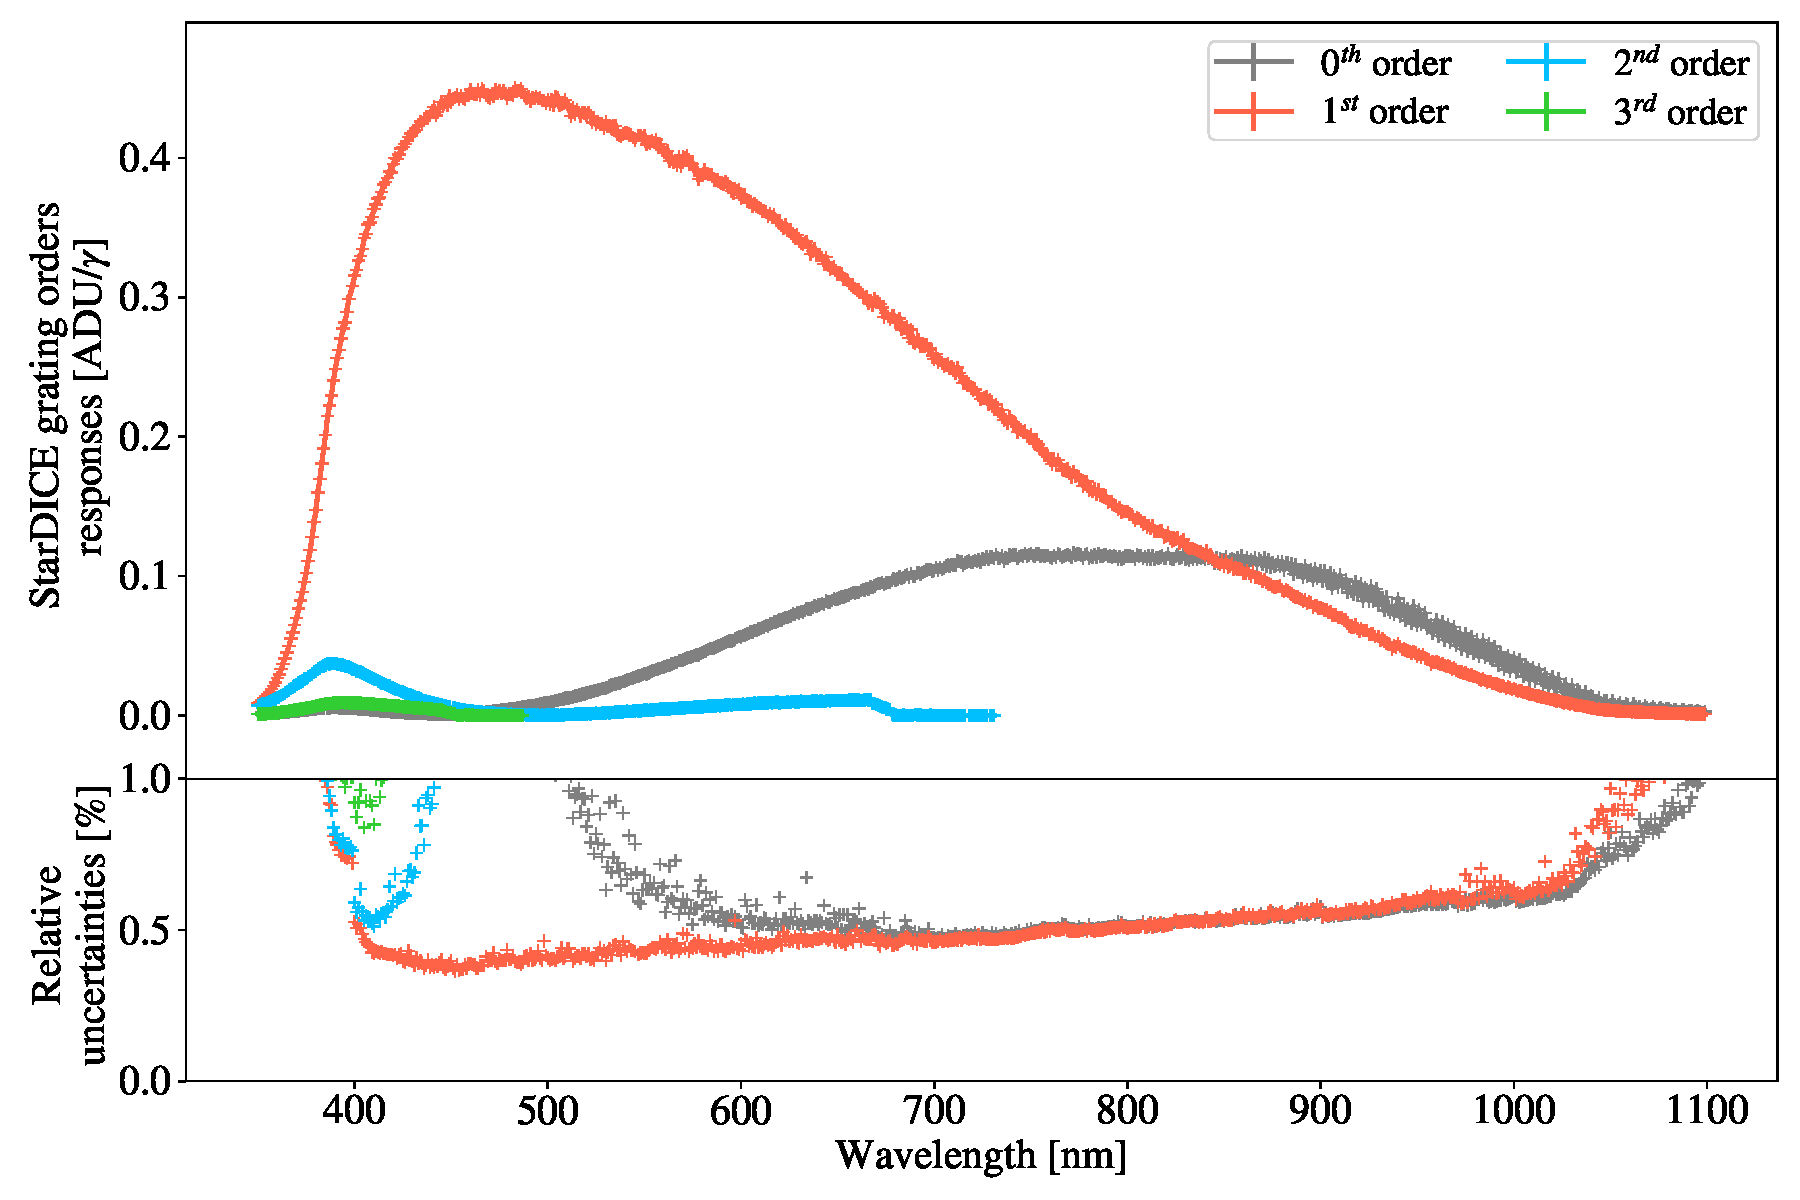
\includegraphics[width=\columnwidth]{fig/stardice_grating_response.pdf}
    \caption{\textit{Top:} \SD response with the grating in front of the camera and \spinhole pinhole with respect to wavelength in nanometer. \textit{Bottom:} Uncertainties over the \SD response measurement with respect to wavelength in nanometer.}
    \label{fig:stardice_grating_response}
    %~/stardice/analysis/cbp_paper/golden_sample_analysis/dr2/response_plots.ipynb
\end{figure}

\subsubsection{Radial positions}

The upper Figure~\ref{fig:radial_positions} show the \SD response obtained with the \spinhole pinhole and without filters for the different radial positions on the mirror shown in Figure~\ref{fig:8_mirror_positions} left, and the same focal plane position. The lower figure shows the relative difference to the mean spline going through the four responses. In the ultraviolet below \SI{450}{\nm}, we can see a significant difference between the four radial positions. It goes up to 30\%, and it will be discussed in the section \ref{sec:discussion}. What we see above \SI{1000}{\nm} in the infrared is the result of the data oscillations around the spline caused by the fringing. 

\begin{figure}[h]
    \centering
    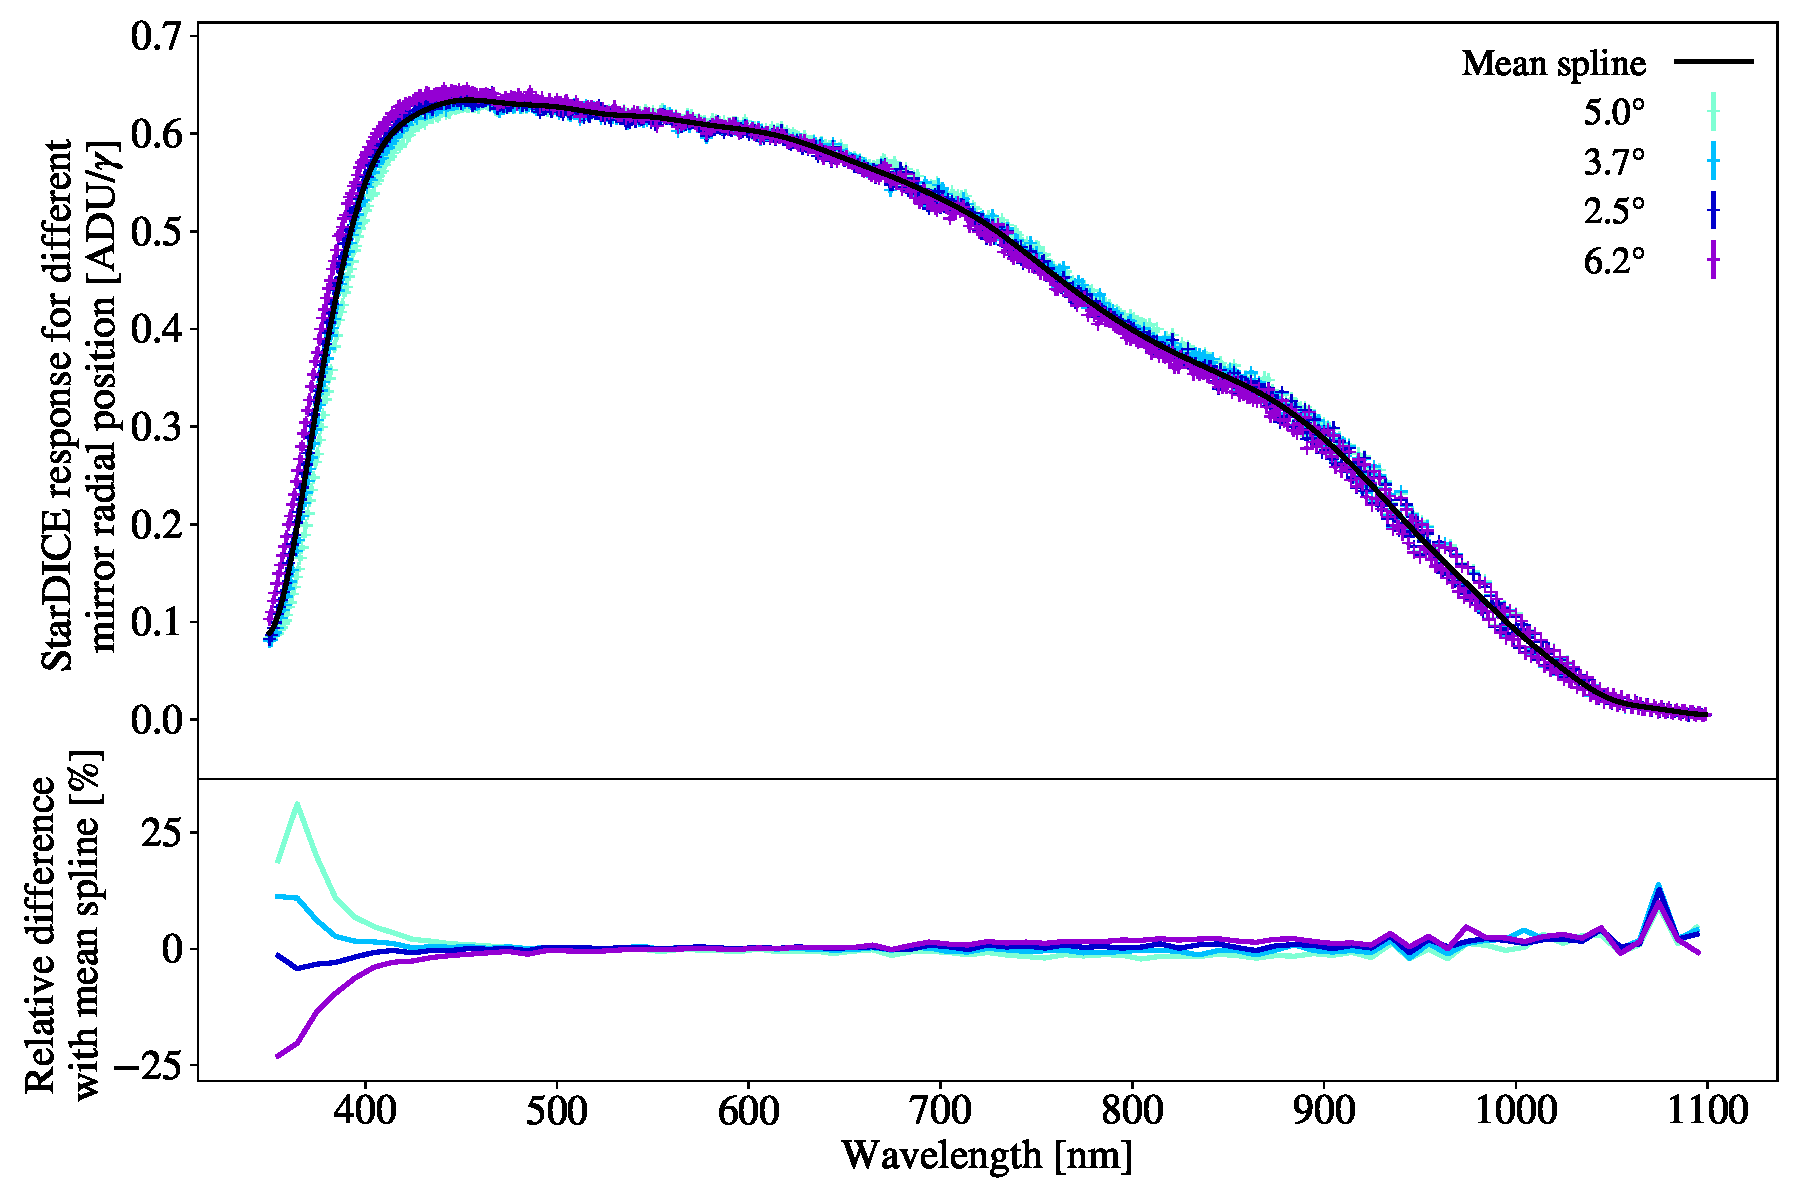
\includegraphics[width=\columnwidth]{fig/radial_positions.pdf}
    \caption{\textit{Top:} \SD response for the different radial positions on the mirror, but same position on the focal plane. \textit{Bottom:} Relative difference between the data and the mean spline.}
    \label{fig:radial_positions}
    %~/stardice/analysis/cbp_paper/golden_sample_analysis/dr2/2022_03_01_stardice_transmission_radius.ipynb
\end{figure}

\subsubsection{Quadrant positions}

The upper Figure~\ref{fig:radial_positions} show the \SD response obtained with the \spinhole pinhole and without filters for the different quadrant positions on the mirror shown in Figure~\ref{fig:8_mirror_positions} right, and the same focal plane position. The lower figure show the normalized residuals to the mean spline going through the four responses. We see again a divergence below \SI{400}{\nm} of about 20\% at most. The phenomenon in the infrared is still caused by the fringing. 

\begin{figure}[h]
    \centering
    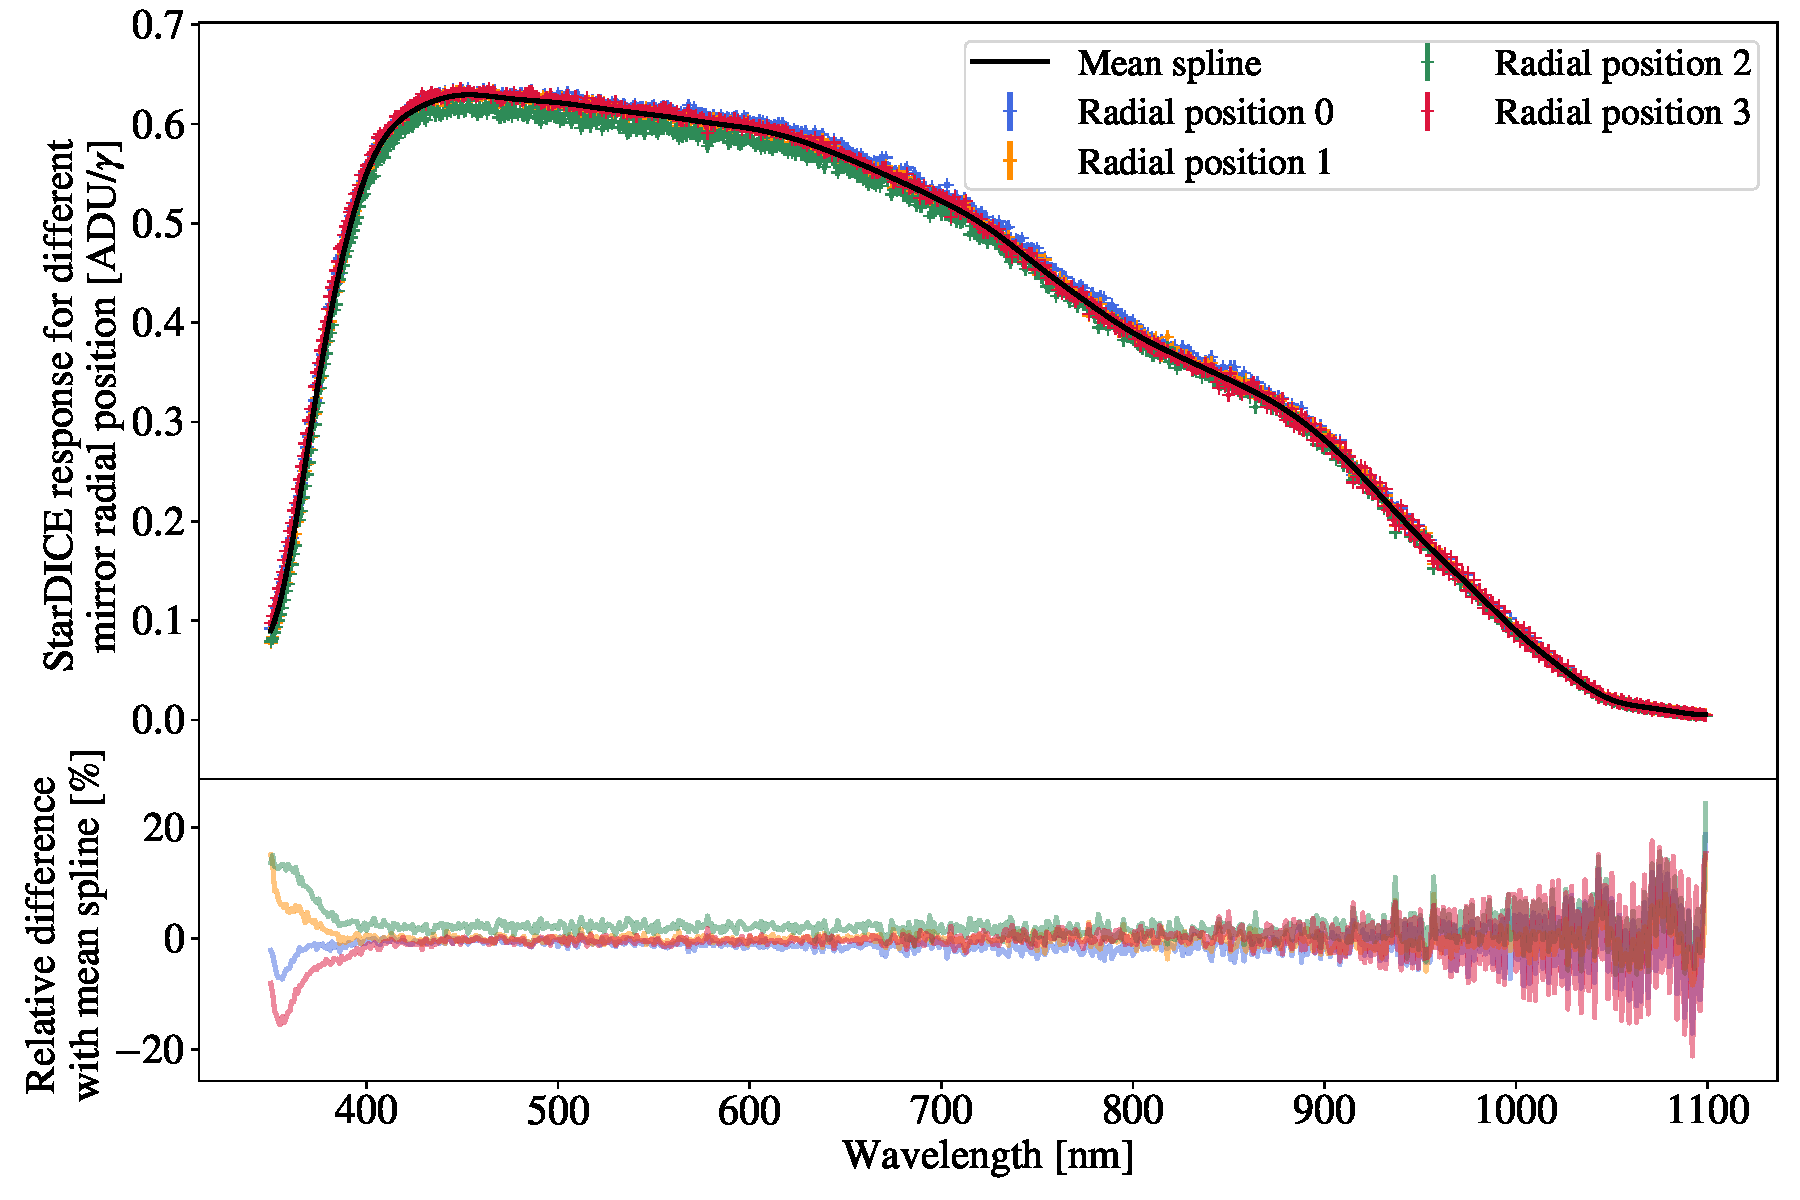
\includegraphics[width=\columnwidth]{fig/quadrant_positions.pdf}
    \caption{\textit{Top:} \SD response for the different quadrant positions on the mirror, but same position on the focal plane. \textit{Bottom:} Relative difference between the data and the mean spline.}
    \label{fig:quadrant_positions}
    %~/stardice/analysis/cbp_paper/golden_sample_analysis/dr2/2022_03_01_stardice_transmission_mirror_samples.ipynb
\end{figure}

\subsubsection{Focal plane positions}

The upper Figure~\ref{fig:ccd_positions} show the \SD response obtained with the \spinhole pinhole and without filters for the same radial and quadrant position on the mirror, and the different focal planes positions from the grid show in Figure~\ref{fig:ccd_grid}. The lower figure show the normalized residuals to the mean spline going through the sixteen responses.

\begin{figure}[h]
    \centering
    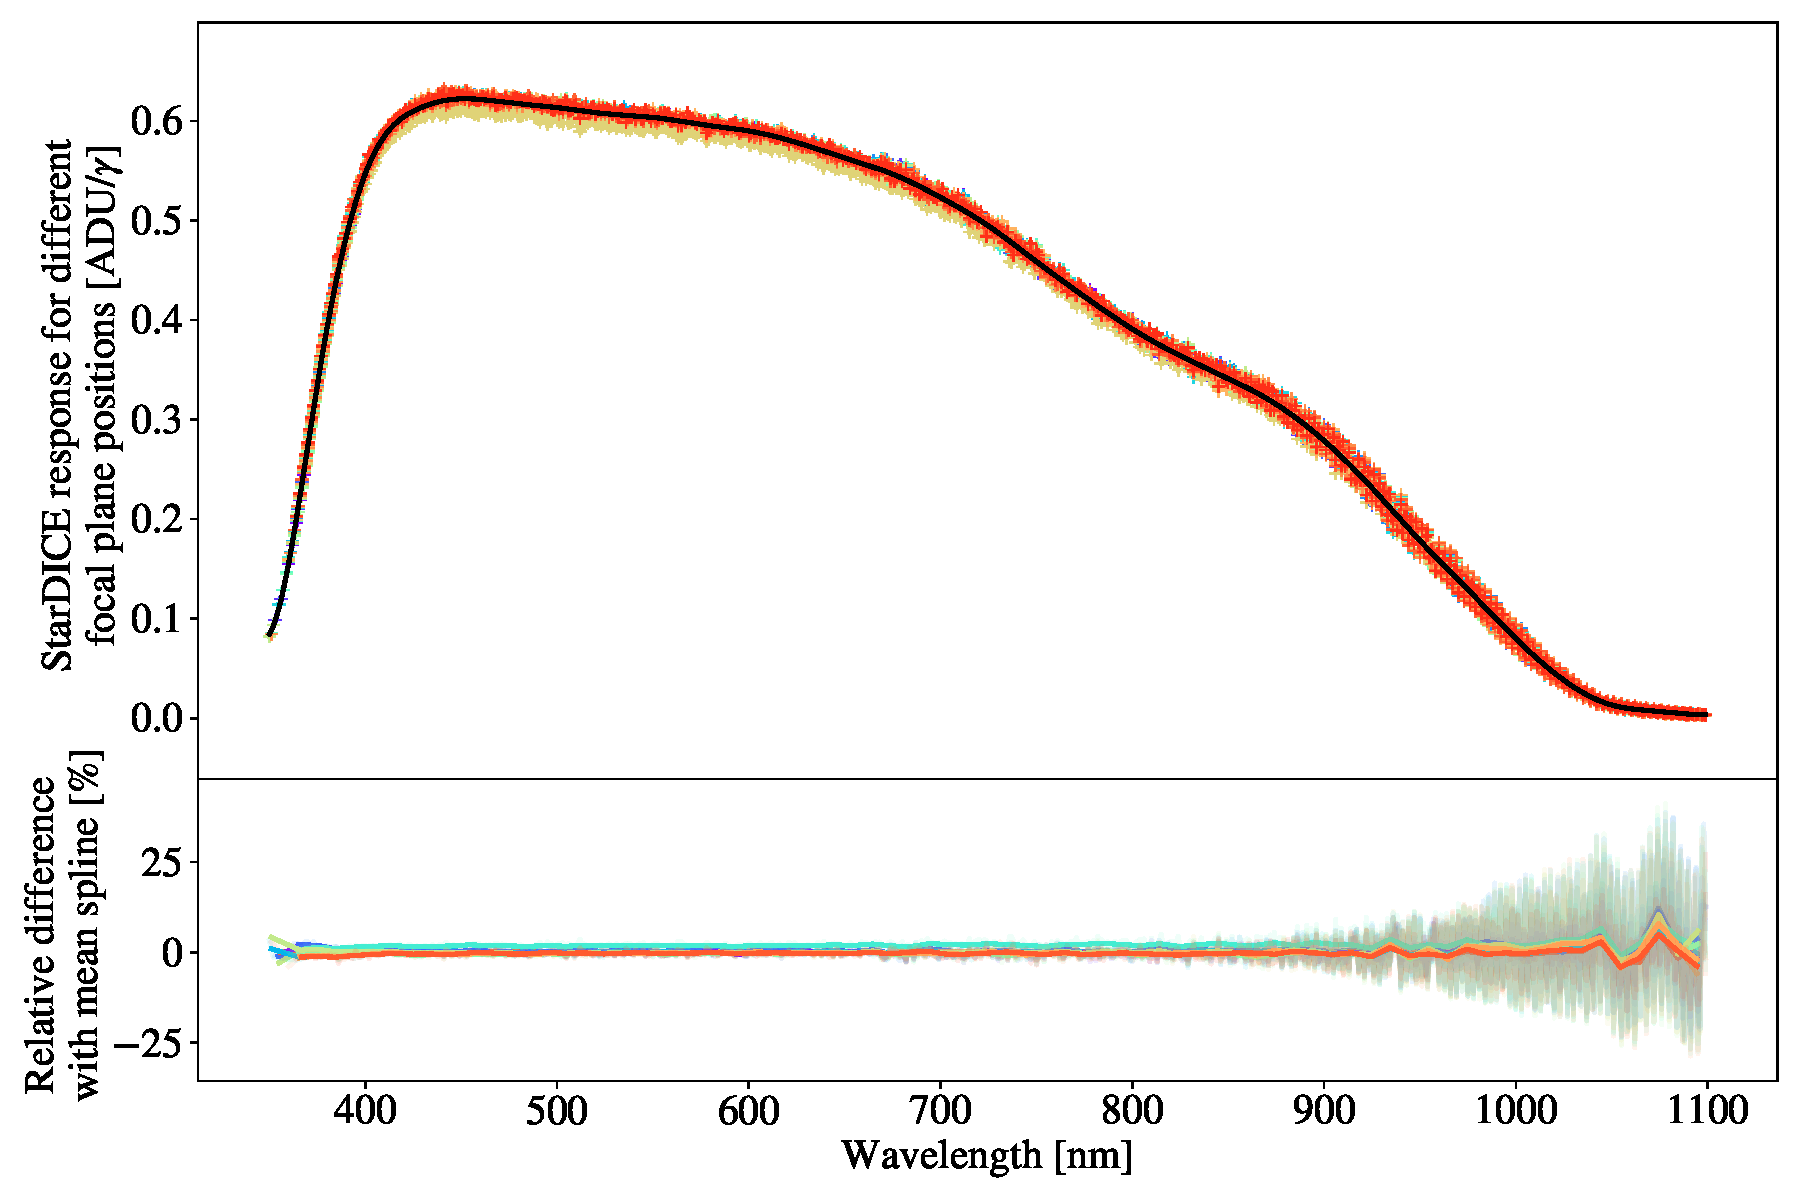
\includegraphics[width=\columnwidth]{fig/ccd_positions.pdf}
    \caption{\textit{Top:} \SD response for the different positions on the focal plane, but same position on the mirror. \textit{Bottom:} Relative difference between the data and the mean spline.}
    \label{fig:ccd_positions}
    %~/stardice/analysis/cbp_paper/golden_sample_analysis/dr2/2022_03_09_stardice_transmission_grid_auto.ipynb
\end{figure}

\subsection{Systematic uncertainties}
\label{sec:systematics}

\subsubsection{Stability of the StarDice responses}

\subsubsection{Gain and linearity}
\label{sec:gain}

Varying pinhole with StarDice, and CBP
Varying QSW but depending on result it falls into this subsection or the following

\subsubsection{Pinhole chromaticity}

\subsubsection{Pull distributions}

\subsubsection{Courbes de croissances}






